\section{Single Phase Full Wave Controlled Rectifier with RL load}

\subsection{Circuit used for simulation}

% figure that is centered on the page
\begin{figure}[h]
    \centering
    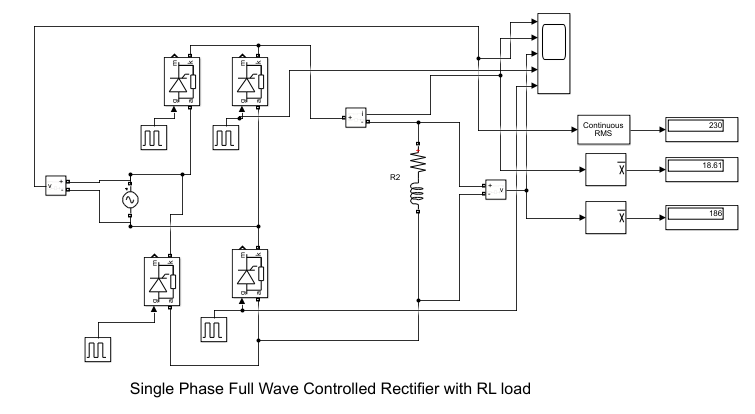
\includegraphics[width=0.7\textwidth]{images/experiment-2/circuit-diagram-simulation-03.png}
    \caption{Circuit used for simulation}
    \label{Fig_simulation_circuit_single-phase-full-wave-controlled-rectifier-with-RL-load}
\end{figure}

\subsection{Components Required}

\begin{table}[h]
    \renewcommand{\arraystretch}{1.3}
    \label{table_components_required_circuit_3}
    \centering
    \begin{tabular}{|c|c|c|c|}
        \hline
        Sr. No & Parameters                     & Ratings            & Quantity \\
        \hline
        \hline
        1      & AC Single Phase Voltage Source & 230V ($ V_{rms} $) & 1        \\
        \hline
        2      & Resistor                       & 10$ \Omega $       & 1        \\
        \hline
        3      & Inductor                       & 10mH               & 1        \\
        \hline
        4      & Diode                          & -                  & 1        \\
        \hline
        5      & Voltmeter                      & -                  & 2        \\
        \hline
        6      & Ammeter                        & -                  & 1        \\
        \hline
    \end{tabular}
    \caption{Components for Single Phase Half Wave Uncontrolled Rectifier with RL load and Freewheeling Diode}
\end{table}


\subsection{Observations}

\begin{table}[h]
    \renewcommand{\arraystretch}{1.3}
    \label{table_observation_3}
    \centering
    \begin{tabular}{|c|c|c|}
        \hline
        Parameters                              & Theoretical Values & Simulation Values \\
        \hline
        \hline
        AC Input Voltage ($ V_{in,rms} $)       & 230V               & 230V              \\
        \hline
        Output Average Voltage ($ V_{o,avg} $)  & 103.53V            & 103V              \\
        \hline
        Output Average Current ($ I_{o,avg}  $) & 10.35A             & 10.3A             \\
        \hline
        AC Input Power ($ P_{AC}  $)            & 2389.5 (W)         & 2266 (W)          \\
        \hline
        DC Input Power ($ P_{DC}  $)            & 1071.53 (W)        & 1015 (W)          \\
        \hline
        Efficiency (\%)                         & 44.84              & 44.8              \\
        \hline
    \end{tabular}
    \caption{Observations for Single Phase Half Wave Uncontrolled Rectifier with RL load and Freewheeling Diode}

\end{table}



It is observed that the simulated values accurately match the theoretical values. On providing gate pulses, the full bridge rectifier, with RL load, shows outputs similar to the half-bridge rectifier with RL load, the former having double the frequency of output voltage and current compared to the latter. Due to the inductive nature of the load, output current lags output voltage, thus delaying the switching off of the thyristors. This results in a momentary negative output voltage, as the thyristors in the rectifier legs briefly allow for the negative half cycle of the AC voltage signal to conduct.
The efficiency of uncontrolled rectifier with RL load with freewheeling diode is 44.8\%.

\pagebreak

\subsection{Resultant Waveforms}


% figure that is centered on the page
\begin{figure}[h]
    \centering
    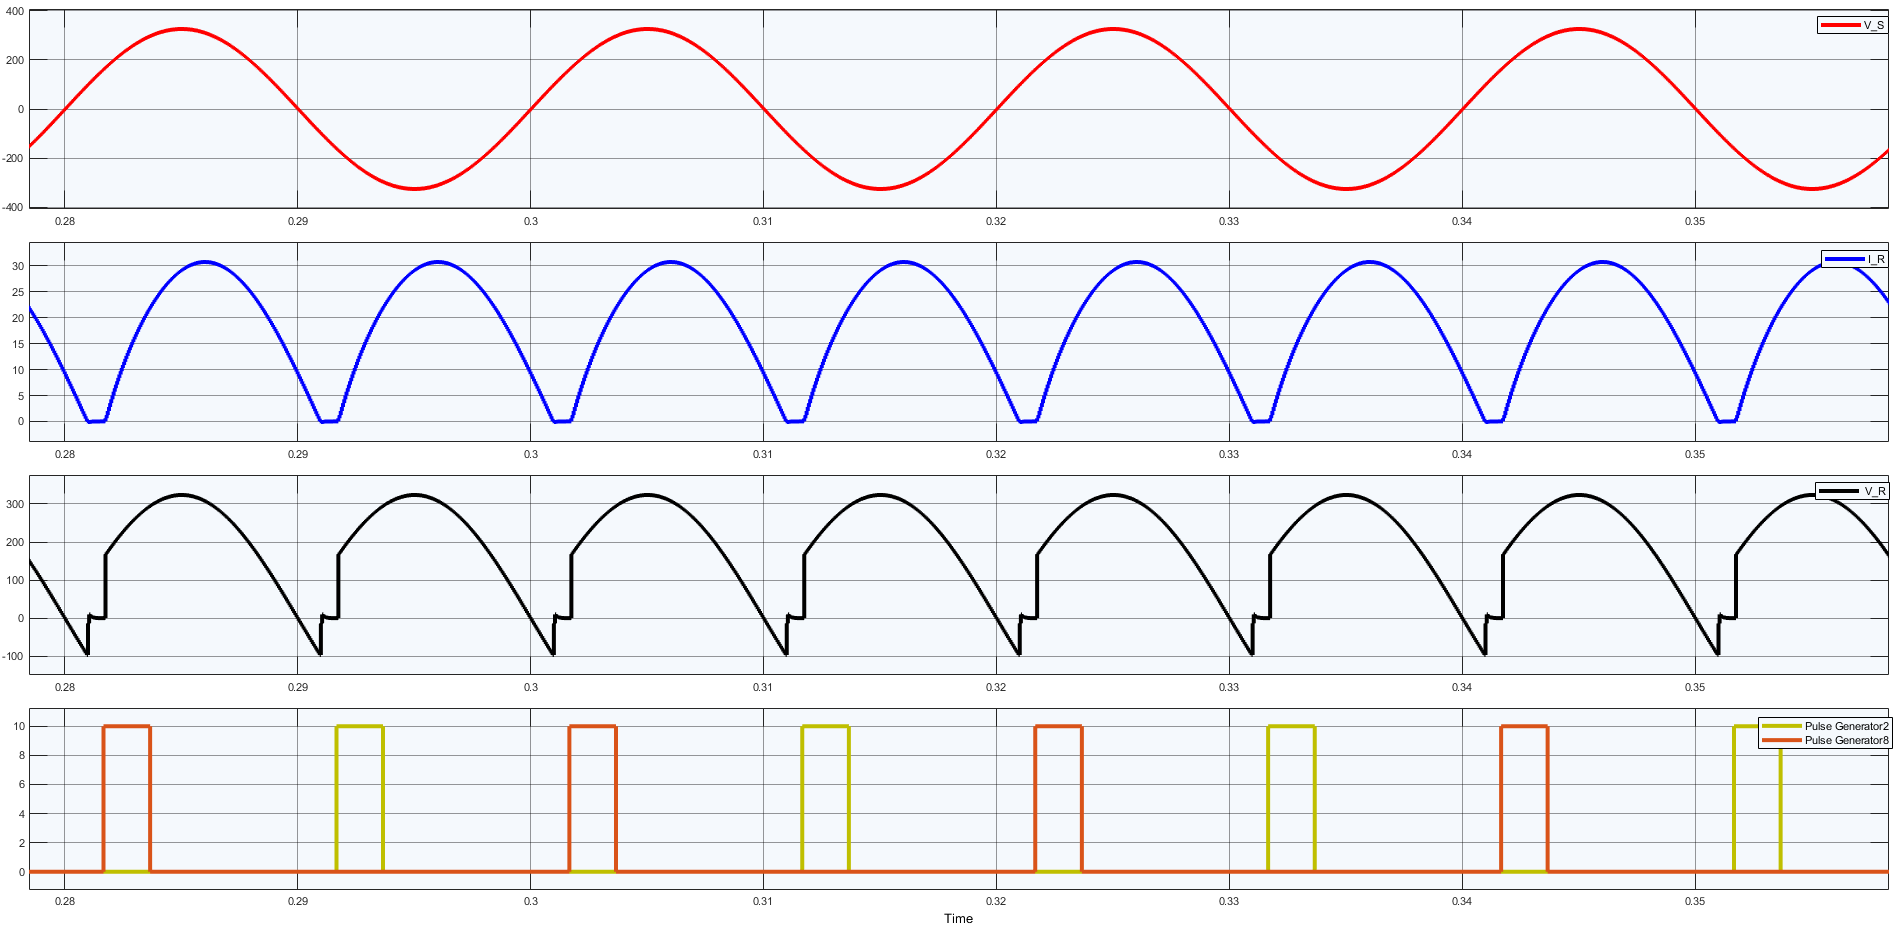
\includegraphics[width=1\textwidth]{images/experiment-2/circuit-scope-simulation-03.png}
    \caption{Scope Waveforms for Single Phase Half Wave Uncontrolled Rectifier with RL load and Freewheeling Diode}
    \label{Fig_waveform_single-phase-full-wave-controlled-rectifier-with-RL-load}
\end{figure}


\pagebreak

